\documentclass{beamer}

\usetheme{default}
\usecolortheme{dolphin}
\beamertemplatenavigationsymbolsempty

\usepackage{tikz}
\usetikzlibrary{
  shapes,
  positioning,
  arrows,
  arrows.meta,
  overlay-beamer-styles, % from aobs-tikz for beamer overlays in tikzpictures
}

\tikzset{
  >={Stealth[width=7pt, length=6pt]},
}

\usepackage{color}
\usepackage{listings}

\definecolor{cc0-green}{RGB}{0, 132, 61}
\definecolor{cc0-yellow}{RGB}{180, 125, 0}
\definecolor{cc0-red}{RGB}{180, 0, 0}
\definecolor{cc0-blue}{RGB}{0, 0, 180}
\definecolor{cc0-gray}{rgb}{0.5,0.5,0.5}

\lstdefinelanguage{C0} {
    language=c,
    commentstyle=\itshape\color{cc0-gray},
    % symbols
    keywords={},
    otherkeywords={!,?},
    keywordstyle=\color{cc0-red},
    % types
    keywordstyle=[2]\color{cc0-blue},
    morekeywords=[2]{int, string, choice, bool, void, struct, enum},
    % C0 keywords
    keywordstyle=[3]\color{cc0-green},
    morekeywords=[3]{if, else, for, while, typedef, switch, case, true, false,
      return, break},
    % CC0 keywords
    keywordstyle=[4]\color{cc0-yellow},
    morekeywords=[4]{send, recv, wait, close},
}

\lstset {
    basicstyle=\ttfamily,
    columns=fixed,
    language=C0,
    basewidth=0.5em,
    escapeinside={{/*\%}{\%*/}}
}

\title[Concurrent C0]{Design and Implementation of Concurrent C0}
\author[M. Willsey, R. Prabhu, F. Pfenning]{
  Max Willsey
  \and
  Rokhini Prabhu
  \and
  Frank Pfenning
}

\institute[]{
  Carnegie Mellon University \\
  School of Computer Science
}
\date{Linearity 2016}

\begin{document}

\frame{\titlepage}

\renewcommand\,{\alt<.(1)>{.}{,}}
\newcommand\blocked{Bar[scale=2, line width=2pt]}
\newcommand\blockedarrow{>Bar[scale=2, line width=2pt]}

\begin{frame}
  \frametitle{Why Concurrent C0?}

  Session types make message passing safer\,
  \pause
  but can they make it more efficient?
  \pause
  {\large\bf Yes!}

  \pause\vspace{2em}

  Session types $\rightarrow$ communication structure $\rightarrow$ efficiency

\end{frame}

\begin{frame}
  \frametitle{Outline}
  \tableofcontents
\end{frame}


\section{Background}
\subsection{Message Passing}

\begin{frame}[fragile]
  \frametitle{Background}
  \framesubtitle{\only<5->{\emph{Asynchronous}} Message Passing}

  \only<-5>{Is 4 even or odd?}
  \only<6-8>{Uh-oh.}
  \only<9>{We need two buffers.}

  \pause\vspace{2em}

  \begin{center}
    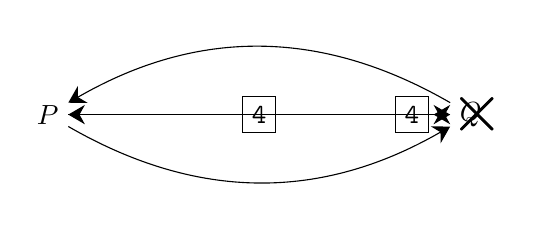
\begin{tikzpicture}[]
      \node (P) {$P$};
      \node (Q) [right=0.4\textwidth of P] {$Q$};
      \pause
      \draw[-,visible on=<+>] (P) to
        (Q);

      \draw[-<,visible on=<+>] (P) to
        node[pos=.9, fill=white, draw] {\texttt{4}}
        (Q);

      \draw[-,visible on=<+>] (P) to
        node[pos=.5, fill=white, draw] {\texttt{4}}
        (Q);

      \draw[->,visible on=<+>] (P) to
        node[pos=.9, fill=white, draw] {\texttt{4}}
        (Q);

      \draw[-,visible on=<+>] (P) to
        node[pos=1.07] {\Huge $\times$}
        (Q);

      \draw[<-,visible on=<+>] (P) to
        node[pos=1.07] {\Huge $\times$}
        (Q);

      \draw[<-,visible on=<+>,bend left]  (P) to (Q);
      \draw[->,visible on=<.>,bend right] (P) to (Q);

    \end{tikzpicture}
  \end{center}
\end{frame}

\subsection{Session Types}
\begin{frame}[fragile]
  \frametitle{Background}
  \framesubtitle{Session Types}

\begin{lstlisting}
typedef <?int; !bool> numberTest;
\end{lstlisting}

\end{frame}

\begin{frame}[fragile]
  \frametitle{Background}
  \framesubtitle{Branching Session Types}

\begin{lstlisting}
typedef <?choice request> atm;
choice request {
    <?amount; !balance; atm>  Deposit;
    <?amount; !choice result> Withdraw;
};
choice result {
    <!payment; atm> Success;
    <atm>           Overdraft;
};
\end{lstlisting}

\end{frame}



\section{Contributions}

\begin{frame}
  \frametitle{Outline}
  \tableofcontents[currentsection]
\end{frame}

\subsection{Synchronization Points}


\begin{frame}[fragile]
  \frametitle{Contributions}
  \framesubtitle{Synchronization Points}

  \begin{center}
    \lstinline+typedef <?int; !bool> numberTest;+
    \vspace{1em}

    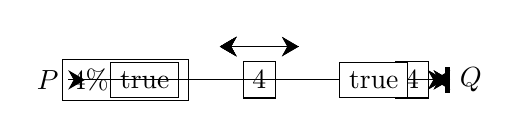
\begin{tikzpicture}[]
      \node (P) {$P$};
      \node (Q) [right=0.4\textwidth of P] {$Q$};
      \draw[-, visible on=<+>] (P) to (Q);

      \draw[-<,visible on=<+>] (P)
        to node[pos=.9, fill=white, draw] {\lstinline+4+}
        (Q);

      \draw[- ,visible on=<+>] (P) to
         node[pos=.5, above=0.5em] {\tikz{\draw[<-] (0,0) to (1,0)}}
         node[pos=.5, fill=white, draw] {\lstinline+4+}
         (Q);

      \draw[->,visible on=<+>] (P) to
         node[pos=.5, above=0.5em] {\tikz{\draw[<-] (0,0) to (1,0)}}
         node[pos=.5, fill=white, draw] {\lstinline+4+}
         (Q);

      \draw[-\blockedarrow,visible on=<+>] (P) to
         node[pos=.5, above=0.5em] {\tikz{\draw[<-] (0,0) to (1,0)}}
         node[pos=.5, fill=white, draw] {\lstinline+4+}
         (Q);

      \draw[<-\blockedarrow, visible on=<+>] (P) to
         node[pos=.5, above=0.5em] {\tikz{\draw[<-] (0,0) to (1,0)}}
         node[pos=.1, fill=white, draw] {\lstinline+4+}
         (Q);

      \draw[-{>Bar[scale=2, line width=2pt]}, visible on=<+>] (P) to
         node[pos=.5, above=0.5em] {\tikz{\draw[<-] (0,0) to (1,0)}}
         node[pos=.15, fill=white, draw] (P') {\lstinline+4\%2==0+}
         (Q);

      \draw[>-{>Bar[scale=2, line width=2pt]},visible on=<+>] (P) to
         node[pos=.5, above=0.5em] {\tikz{\draw[->] (0,0) to (1,0)}}
         node[pos=.2, fill=white, draw] {\lstinline+true+}
         (Q);

      \draw[->,visible on=<+>] (P) to
         node[pos=.5, above=0.5em] {\tikz{\draw[->] (0,0) to (1,0)}}
         node[pos=.8, fill=white, draw] {\lstinline+true+}
         (Q);
    \end{tikzpicture}

    \hfill
    \begin{minipage}[t]{0.4\linewidth}
      \alert<6>{\texttt{int x = recv(\$c);} \\}%
      \alert<8>{\texttt{send(\$c, x\%2==0);} \\}%
    \end{minipage} \hfill %
    \begin{minipage}[t]{0.35\linewidth}%
      \alert<2>{\texttt{send(\$c, 4);} \\}%
      \alert<4->{\texttt{recv(\$c);} \\}%
    \end{minipage}
    \hfill
  \end{center}
\end{frame}

\subsection{Type Width}

\begin{frame}[fragile]
  \frametitle{Contributions}
  \framesubtitle{Type Width}

  \small

  \begin{overlayarea}{\textwidth}{0.4\textheight} \centering
  \begin{onlyenv}<1-3>
  \vspace{-1em}
  \begin{lstlisting}
typedef <?choice request> atm;
choice request {
    <?amount; !balance; atm>  Deposit;
    <?amount; !choice result> Withdraw;
};
choice result {
    <!payment; atm> Success;
    <atm>           Overdraft;
};
  \end{lstlisting}
  \end{onlyenv}
  \begin{onlyenv}<4-5>
  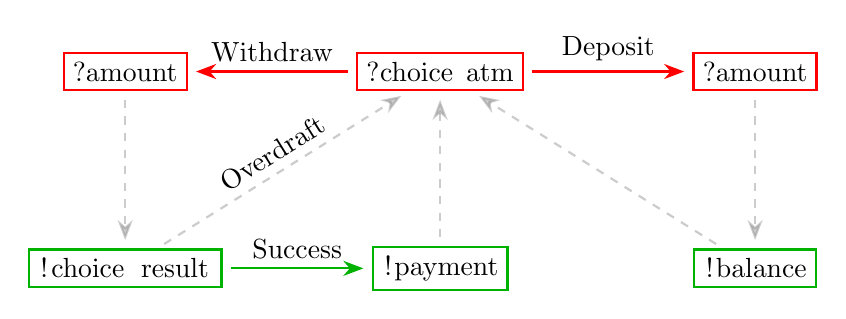
\begin{tikzpicture}[
      x=4cm, y=2.5cm,
      thick,
      -{Stealth[scale=1.1]}, shorten >=3pt, shorten <=3pt,
      send/.style={draw=black!30!green},
      recv/.style={draw=red},
      sync/.style={draw=gray, dashed, opacity=0.4}]

    \node[recv] (atm)             at (0, 0) {\lstinline+?choice atm+};
    \node[recv] (Deposit-amount)  at (1, 0) {\lstinline+?amount+};
    \node[recv] (Withdraw-amount) at (-1,0) {\lstinline+?amount+};
    \node[send] (result)          at (-1,-1) {\lstinline+!choice result+};
    \node[send] (Success-payment) at (0,-1) {\lstinline+!payment+};
    \node[send] (Deposit-balance) at (1,-1) {\lstinline+!balance+};

    \path[anchor=south]
      (atm)             edge[recv] node  {\lstinline+Deposit+}  (Deposit-amount)
                        edge[recv] node  {\lstinline+Withdraw+} (Withdraw-amount)
      (Deposit-amount)  edge[sync]                                (Deposit-balance)
      (Deposit-balance) edge[sync]                                (atm)
      (Withdraw-amount) edge[sync]                                (result)
      (Success-payment) edge[sync]                                (atm)
      (result)          edge[send] node {\lstinline+Success+}  (Success-payment)
                        edge[sync]
                        node[sloped, draw=none, opacity=1] {\lstinline+Overdraft+} (atm);
  \end{tikzpicture}
  \end{onlyenv}
  \end{overlayarea}

  \begin{center}
    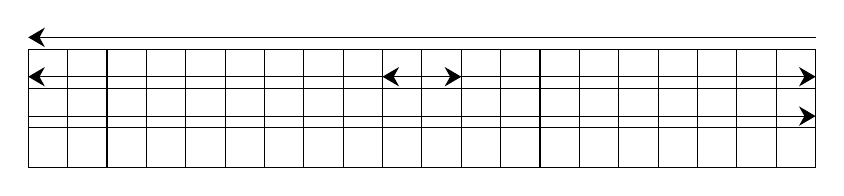
\begin{tikzpicture}
      \draw[<-, visible on=<2>] (0,1.65) to (10,1.65);
      \draw[step=5mm, visible on=<2>] (0,0) grid (10,0.5);
      \draw[->, visible on=<2>] (0,0.65) to (10,0.65);
      \draw[step=5mm, visible on=<2>] (0,0.999) grid (10,1.5);
      \draw[<->, visible on=<3-4>] (0,1.15) to (10,1.15);
      \draw[step=5mm, visible on=<3-4>] (0,0.5) grid (10,1);
      \draw[<->, visible on=<5>] (4.499,1.15) to (5.5,1.15);
      \draw[step=5mm, visible on=<5>] (4.499,0.5) grid (5.5,1);
    \end{tikzpicture}
  \end{center}
\end{frame}

\subsection{Forwarding}
\begin{frame}[fragile]
  \frametitle{Contributions}
  \framesubtitle{Forwarding}

  \begin{center}

  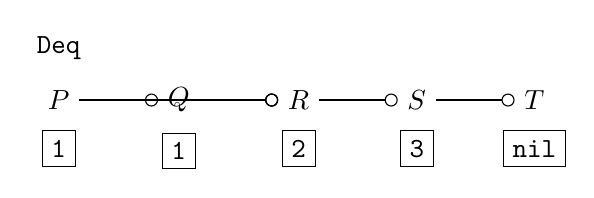
\begin{tikzpicture}
    \node (P) {$P$};
    \node (Q) [right=of P, visible on=<-5>] {$Q$};
    \node (R) [right=of Q] {$R$};
    \node (S) [right=of R] {$S$};
    \node (T) [right=of S] {$T$};

    \node (Deq) [above=0.4em of P, visible on=<3-4>] {\texttt{Deq}};

    \node (1)   [below=0.4em of Q, visible on=<2-3>, draw] {\texttt{1}};
    \node (1)   [below=0.4em of P, visible on=<4->, draw] {\texttt{1}};
    \node (2)   [below=0.4em of R, visible on=<2->, draw] {\texttt{2}};
    \node (3)   [below=0.4em of S, visible on=<2->, draw] {\texttt{3}};
    \node (nil) [below=0.4em of T, visible on=<2->, draw] {\texttt{nil}};

    \draw[-o, visible on=<-6>] (P) to (Q);
    \draw[-o, visible on=<-6>] (Q) to (R);
    \draw[-o, visible on=<7->] (P) to (R);

    \draw[-o] (Q) to (R);
    \draw[-o] (R) to (S);
    \draw[-o] (S) to (T);
  \end{tikzpicture}

  \end{center}
\end{frame}

\begin{frame}[fragile]
  \frametitle{Contributions}
  \framesubtitle{Forwarding as a message}

  \begin{center}

  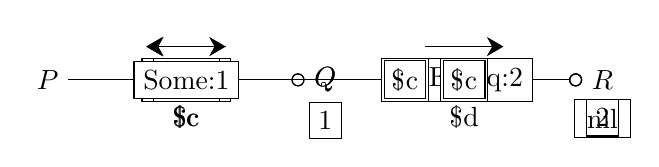
\begin{tikzpicture}
    \node (P) {$P$};
    \node[visible on=<-2>] (Q) [right=3cm of P] {$Q$};
    \node (R) [right=3cm of Q] {$R$};

    \draw[-o, visible on=<-2>] (P) to (Q);
    \draw[-o, visible on=<-2>] (Q) to (R);
    \draw[-o, visible on=<7>]  (P) to
      node[pos=.228, above=0.5em] {\tikz{\draw[<-] (0,0) to (1,0)}}
      node[pos=.228, fill=white, draw] {\lstinline+Some:1+}
      node[pos=.228, below=2mm] {\lstinline+$c+}
      (R);

    \node[visible on=<1-4>] (Q) [right=3cm of P] {$Q$};
    \node[draw, visible on=<1-3>] (Q1) [below=0em of Q] {\lstinline+1+};
    \node[draw, visible on=<1-5>] (R1) [below=0em of R] {\lstinline+nil+};
    \node[draw, visible on=<6->]  (R1) [below=0em of R] {\lstinline+2+};

    \draw[-o, visible on=<1-6>] (P) to
      node[pos=.5, above=0.5em, visible on=<-3>] {\tikz{\draw[->] (0,0) to (1,0)}}
      node[pos=.5, above=0.5em, visible on=<4->] {\tikz{\draw[<-] (0,0) to (1,0)}}
      node[pos=.5, fill=white, draw, visible on=<1>] {\lstinline+Enq:2+}
      node[pos=.5, fill=white, draw, visible on=<3>] {\lstinline+Deq+}
      node[pos=.5, fill=white, draw, visible on=<4->] {\lstinline+Some:1+}
      node[below=2mm] {\lstinline+$c+}
      (Q);
    \draw[-o, visible on=<1-6>] (Q) to
      node[pos=.5, above=0.5em] {\tikz{\draw[->] (0,0) to (1,0)}}
      node[pos=.5, fill=white, draw, visible on=<2-4>] {\lstinline+Enq:2+}
      node[pos=.25, fill=white, draw, double, visible on=<5>] {\lstinline+$c+}
      node[pos=.6, fill=white, draw, visible on=<5>] {\lstinline+Enq:2+}
      node[pos=.5, fill=white, draw, double, visible on=<6>] {\lstinline+$c+}
      node[below=2mm] {\lstinline+$d+}
      (R);
  \end{tikzpicture}

  \end{center}
\end{frame}

\section{Results}
\subsection{Benchmarks}

\begin{frame}
  \frametitle{Results}

  It works!

  \pause\vspace{1em}

  Compiler in SML

  \pause\vspace{1em}

  Runtimes in C and Go

  \pause\vspace{1em}

  \tiny *See extended version of paper

\end{frame}


\begin{frame}
  \frametitle{Results}
  \framesubtitle{Benchmarks}

  \begin{center}
  Concurrent C0 implemented in Go with optimizations \\
  \pause
  vs. \\
  Conventional Go message passing

  \pause\vspace{1em}

    {\huge $1.38\times$ faster}

    \pause\vspace{1em}

    \includegraphics[width=\textwidth]{go02benchmarks}
  \end{center}

\end{frame}

\begin{frame}
  \frametitle{Takeaways}

  Session types give valuable insight into the structure of communication that's
  useful for safety \alert<+(1)>{and efficient implementation}.

  \pause \vspace{1em}

  Session types $\rightarrow$ memory-saving optimizations

  \pause \vspace{1em}

  \textbf{Future work:} Session types $\rightarrow$ scheduling?

\end{frame}

\end{document}